
\documentclass[main.tex]{subfiles}

\begin{document}

\section{基本初等复合函数的积分}

虽然基本初等函数的积分很简单,基本初等函数经过四则运算再积分也可以写出初等表达式,但是基本初等函数的复合函数的积分可能就不存在初等表达式。以下列出几个,重点在于这些函数的定积分的值。
\begin{itemize}
    \item[(1)] 菲涅尔积分(Fresnel integral)
    \[ \trm{S}(x) = \int_{0}^{x} \sin(t^2)\trm{d} t \quad \mbox{和} \quad \trm{C}(x) = \int_{0}^{x} \cos(t^2)\trm{d} t\]
% \pgfdeclarelayer{nodelayer}
% \pgfdeclarelayer{edgelayer}
% \pgfsetlayers{nodelayer, edgelayer}
% \begin{center}
% \begin{tikzpicture}
% 	\begin{pgfonlayer}{nodelayer}
% 		\node (0) at (0, 0) {};
% 		\node (1) at (5, 0) {};
% 		\node (2) at (4, 3) {};
% 	\end{pgfonlayer}
% 	\begin{pgfonlayer}{edgelayer}
% 		\draw (0.center) to (2.center);
% 		\draw (0.center) to (1.center);
% 		\draw [bend right] (1.center) to (2.center);
% 	\end{pgfonlayer}
% \end{tikzpicture}
% \end{center}
    \item[(2)] 三角函数和双曲函数积分\\
% \begin{wrapfigure}{r}{4cm}%靠文字内容的左侧
%     \centering
%     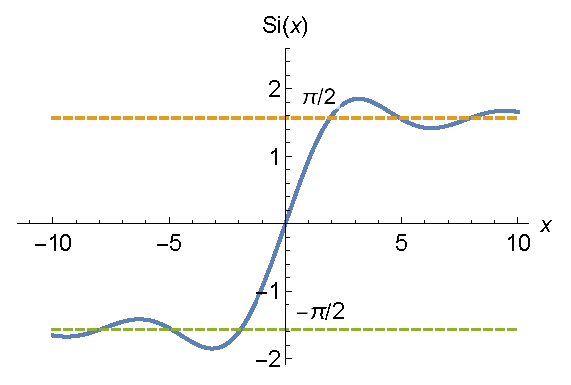
\includegraphics[width=0.3\textwidth]{si.eps}
%     \caption{\footnotesize 正弦积分}
% \end{wrapfigure}
    \begin{equation*}
        \begin{array}{ll}
            \displaystyle{\trm{sinc}(x) = \frac{\sin(x)}{x}} &
            \displaystyle{\trm{Si}(x) = \int_{0}^{x} \trm{sinc}(t) \trm{d}t}  \\
            \displaystyle{\trm{cosc}(x) = \frac{\cos(x)}{x}} &
            \displaystyle{\trm{Ci}(x) = \int_{0}^{x} \trm{cosc}(t) \trm{d}t}  \\
            \displaystyle{\trm{sinhc}(x) = \frac{\sinh(x)}{x}} &
            \displaystyle{\trm{Shi}(x) = \int_{0}^{x} \trm{sinhc}(t) \trm{d}t}  \\
            \displaystyle{\trm{coshc}(x) = \frac{\cos(x)}{x}} &
            \displaystyle{\trm{Chi}(x) = \int_{0}^{x} \trm{coshc}(t) \trm{d}t}  \\
        \end{array}
    \end{equation*}
% \begin{figure}[H]
%    \centering
%    \subfigure[]{
%        \label{fig:a} %% label for first subfigure
%        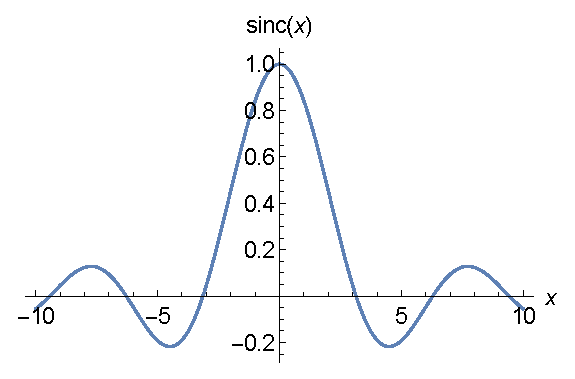
\includegraphics[width=0.32\textwidth]{sinc.eps}
%    }
%    \subfigure[]{
%        \label{fig:b} %% label for secondsubfigure
%        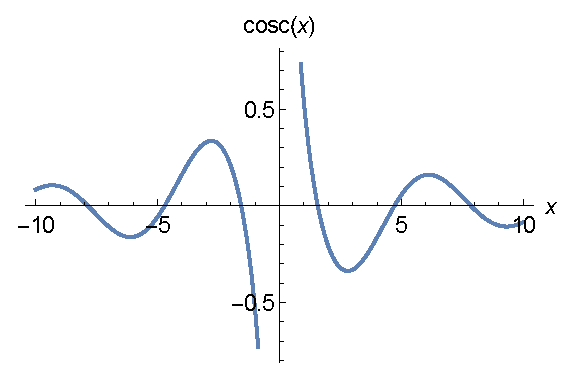
\includegraphics[width=0.32\textwidth]{cosc.eps}
%    }
% \end{figure}
% \begin{figure}[H]
%     \centering
%    \subfigure[]{
%        \label{fig:c} %% label for secondsubfigure
%        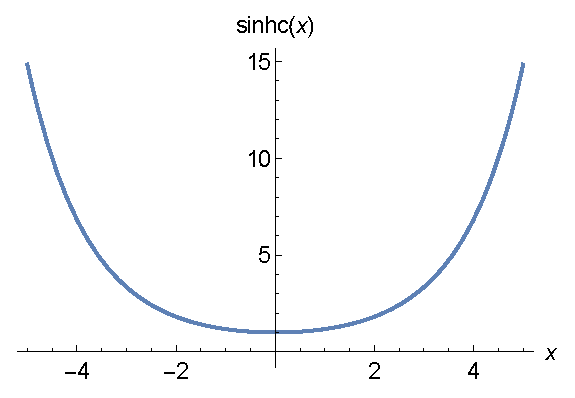
\includegraphics[width=0.32\textwidth]{sinhc.eps}
%    }
%    \subfigure[]{
%        \label{fig:d} %% label for secondsubfigure
%        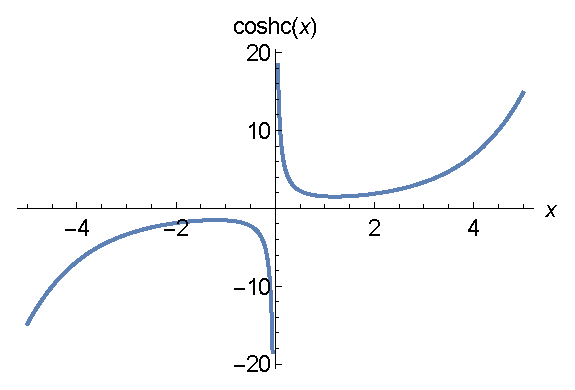
\includegraphics[width=0.32\textwidth]{coshc.eps}
%    }
%    \caption{composited function}
%    \label{figb} %% label for entire figure
% \end{figure}
    \item[(3)] 指数积分(exponentiation integral)
    \[ \trm{Ei}(x) = \int_{0}^{x} \frac{e^{-t}}{t} \trm{d}t \]
    \item[(4)] 对数积分(logarithm integral)
    \[ \trm{li}(x) = \int_{0}^{x} \frac{\ln(t)}{t} \trm{d}t \]
\end{itemize}

\section{柱函数(贝塞尔函数)系}

\subsection{为什么会有这个函数?}

回顾线性代数的知识:
\begin{reference}
    在线性空间\(\langle S;+,\cdot \rangle\)中定义一个映射\(f\),对于任意常数\(a,b\),如果该变换满足
    \[f(ax+by)=af(x)+bf(y)\]
    就称该映射具有\uline{线性}。更进一步地,如果存在向量\(x\),使得存在常数\(\lambda\),满足\(f(x)=\lambda x\),则称该\(\lambda\)为该映射的\uline{特征值},\(x\)称为该映射对应于\(\lambda\)的\uline{特征向量}.
\end{reference}

我们知道二维平面上的拉普拉斯算子\(\displaystyle{\nabla^2 =\frac{\partial^2}{\partial x^2}+\frac{\partial^2 }{\partial y^2}}\)是\(\mathbb{R}^3\)上的线性映射(不信你自己验证).自然地,二维向量的特征值就应该满足
\[\nabla^2 f(x,y)=\lambda f(x,y)\]
这个式子称为\uline{亥姆霍兹方程}(Helmholtz equation). 亥姆霍兹方程在物理学中经常用到,它的解(也就是特征值)有无数多个. 换个坐标系,根据极坐标系和直角坐标系的关系:
\[\rho = \sqrt{x^2+y^2} \qquad \theta = \arg(x+iy)\]
将拉普拉斯算子改写为极坐标的形式:
\[\nabla^2 = \frac{1}{\rho}\frac{\partial}{\partial \rho}\left(\rho\frac{\partial}{\partial \rho}\right) + \frac{1}{\rho^2}\frac{\partial^2}{\partial \theta^2} = \rho\frac{\partial^2}{\partial \rho^2} + \frac{1}{\rho}\frac{\partial}{\partial \rho^2} + \frac{1}{\rho^2}\frac{\partial^2}{\partial \theta^2}\]
根据\uline{分离变量}(separation of variables)的思想,假设函数\(f(\rho,\theta)\)能被写成两个单变量函数的乘积:\(f(\rho,\theta)\equiv R(\rho)T(\theta)\),亥姆霍兹方程就可以改写成这个形式(将\(R(\rho)\)简写为\(R\),\(T(\theta)\)简写为\(T\)):
\[R''T+\frac{1}{\rho}R'T+\frac{1}{\rho^2}RT''=\lambda RT\]
两边乘以\(\rho^2\),再除以\(RT\),得到
\[\rho^2\frac{R''}{R}+\rho\frac{R'}{R}+\frac{T''}{T}=\lambda\rho^2\]
左边是三个单项式相加的形式,其中参数\(\theta\)只与第三个单项式\(\displaystyle{\frac{T''(\theta)}{T(\theta)}}\)有关,然而右边却与\(\theta\)无关,这说明\(\displaystyle{\frac{T''(\theta)}{T(\theta)}}\)必须是一个常数,否则当\(\theta\)发生变化后,左边的值就会发生变化,而这种变化是与\(\theta\)无关的参数\(\rho\)所无法抵消的. 所以设\(\displaystyle{\frac{T''(\theta)}{T(\theta)} = \mu}\),这是一个很好解的常微分方程,再看另外一边:
\[\rho^2\frac{R''}{R}+\rho\frac{R'}{R}+\mu=\lambda\rho^2\]
两边乘\(R\),整理一下得到
\[\rho^2 R''+\rho R'+ (\mu-\lambda\rho^2)R = 0\]
这个微分方程称为\uline{贝塞尔方程},它的解不一定能表示为初等形式,由其隐式定义的函数称为\uline{贝塞尔函数}(Bessel function).

\begin{definition}{贝塞尔函数}
    微分方程
    \[x^2y″ + xy′ + (x^2-\alpha^2)y = 0\]
    的解称为\(\alpha\)阶的贝塞尔函数,记作\(J_\alpha(x)\),其中\(x\)称为\uline{宗量},阶数和宗量的范围为复数集.
\end{definition}

再换一种坐标系. 在三维空间,拉普拉斯算子为\(\displaystyle{\nabla^2 = \frac{\partial^2}{\partial x^2}+\frac{\partial^2}{\partial y^2}+\frac{\partial^2}{\partial z^2}}\). 根据球坐标系与直角坐标系的关系:
\[r = \sqrt{x^2+y^2+z^2} \qquad \theta = \arg(x+iy) \qquad \varphi = \arccos(z/r)\]
将拉普拉斯算子改写为球坐标的形式,得到一个非常难看的式子:
\[\nabla^2 = \frac{1}{r^2}\frac{\partial}{\partial r}\left(r^2 \frac{\partial}{\partial r}\right)+\frac{1}{r^2\sin^2\theta}\frac{\partial}{\partial \theta}\left(\sin\theta \frac{\partial}{\partial \theta}\right)+\frac{1}{r^2\sin^2\theta}\frac{\partial^2}{\partial \varphi^2}\]
就像上面那样,根据分离变量的思想,假设函数\(f(r,\theta, \varphi)=R(r)T(\theta)P(\varphi)\),代入亥姆霍兹方程:
\[\frac{TP}{r^2}\left(r^2 R'\right)'+\frac{RP}{r^2\sin^2\theta}\left(T'\sin\theta\right)'+\frac{RT}{r^2\sin^2\theta}P''=\lambda RTP\]
两边同除\(RTP\),再乘以\(r^2\),得到
\[\frac{\left(r^2 R'\right)'}{R}+\frac{\left(T'\sin\theta\right)'}{T\sin^2\theta}+\frac{P''}{P\sin^2\theta} = \lambda r^2\]
左侧是三个单项式,注意其中的第二、第三个单项式与\(r\)无关,基于相同理由,我们又可以把它设为常数\(\mu\),于是这就出来了一个单变量的微分方程,将括号展开:
\[r^2R''+2rR'+(\mu-\lambda r^2)R = 0\]
这个微分方程称为\uline{球贝塞尔方程},它的解不一定能表示为初等形式,由其隐式定义的函数称为\uline{球贝塞尔函数}(spherical Bessel function).

\begin{definition}{球贝塞尔函数}
    微分方程
    \[x^2y″ + xy′ + (x^2-\alpha^2)y = 0\]
    的解称为\(\alpha\)阶的贝塞尔函数,记作\(J_\alpha(x)\),其中\(x\)称为\uline{宗量},阶数和宗量的范围为复数集.
\end{definition}

\subsection{解贝塞尔方程:Frobenius法}

我们知道二阶、线性、齐次、常系数的微分方程怎么解,但是把“常系数”去掉呢?就会解出一大堆特殊函数,可以说博物馆中的所有特殊函数都可以通过解这样的方程得到.

% \begin{itemize}
%     \item[(1)] 拉普拉斯方程为\(\nabla^2 u =0\),根据柱坐标系与直角坐标系的关系:
%     \[\rho = \sqrt{x^2+y^2} \qquad \theta = \arg(x+iy) \qquad z = z\]
%     在三维柱坐标系下展开得到
%     \[\frac{1}{\rho}\frac{\partial}{\partial \rho}\left(\rho\frac{\partial u}{\partial \rho}\right) + \frac{1}{\rho^2}\frac{\partial^2 u}{\partial \theta^2} + \frac{\partial^2 u}{\partial z^2} = 0\]
%     分离变量,令\(u(\rho,\theta,z)=f(\rho)g(\theta)h(z)\),回代并在等号两边同时乘以\(\displaystyle{\frac{r^2}{f(\rho)g(\theta)h(z)}}\),得到
%     \[\frac{\rho}{f(\rho)}\frac{\partial}{\partial \rho}\left(\rho f'(\rho)\right) + \frac{g''(\theta)}{g(\theta)} + \rho^2\frac{h''(z)}{h(z)} = 0\]
%     左边是三个单项式相加的形式,其中参数\(\theta\)只与第二个单项式\(\displaystyle{\frac{g''(\theta)}{g(\theta)}}\)有关,然而右边为常数\(0\),这说明\(\displaystyle{\frac{g''(\theta)}{g(\theta)}}\)必须是一个常数,否则当\(\theta\)发生变化后,左边的值就会发生变化,而这种变化是与\(\theta\)无关的参数\(\rho,z\)所无法抵消的. 所以设\(\displaystyle{\frac{g''(\theta)}{g(\theta)}} = -n^2\),回代的同时两边同除\(r^2\),得到
%     \[\frac{1}{\rho f(\rho)}\frac{\partial}{\partial \rho}\left(\rho f'(\rho)\right) -\frac{n^2}{r^2} + \frac{h''(z)}{h(z)} = 0\]
%     对\(\displaystyle{\frac{h''(z)}{h(z)}}\)使用相同的手法,令其为\(k_z^2\),回代的同时两边再同乘\(f(\rho)\),得到
%     \[\frac{1}{\rho}\frac{\partial}{\partial \rho}\left(\rho f'(\rho)\right) + \left(k_z^2-\frac{n^2}{\rho^2}\right)f(\rho) = 0\]
%     两边同乘\(r^2\)整理得到
%     \[\rho^2f''(\rho)+rf'(\rho)+[(k_z\rho)^2-n^2]f(\rho) = 0\]
%     这就得到了贝塞尔方程.

%     \item[(2)] 热传导方程为\(\displaystyle{\frac{\partial u}{\partial t} = a^2\nabla^2 u}\),在二维
%     \item[] 
% \end{itemize}

\begin{definition}{贝塞尔函数}
    第一类贝塞尔函数
    \[J_{\alpha}(x) = \sum_{n=0}^{\infty} \frac{(-1)^{n}}{n!\Gamma (n+\alpha +1)}{\left({\frac {x}{2}}\right)}^{2n+\alpha}\]
    第二类贝塞尔函数
    \[Y_{\alpha}(x) = \frac{J_{\alpha}(x)\cos(\alpha\pi)-J_{-\alpha}(x)}{\sin(\alpha\pi)}\]
    汉克尔函数
    \[
        \begin{aligned}
            H_{\alpha }^{(1)}(x) &= J_{\alpha }(x)+iY_{\alpha }(x) \\ 
            H_{\alpha}^{(2)}(x) &= J_{\alpha}(x)-iY_{\alpha}(x) 
        \end{aligned}
    \]
    修正贝塞尔函数
    \[
        \begin{aligned}
            I_{\alpha }(x) &= i^{-\alpha }J_{\alpha }(ix) \\
            K_{\alpha }(x) &= \frac {\pi }{2}{\frac {I_{-\alpha }(x)-I_{\alpha }(x)}{\sin \alpha \pi }} 
        \end{aligned}
    \]
    球贝塞尔函数
    \[
        \begin{aligned}
            j_{n}(x) &= \sqrt{\frac {\pi }{2x}}J_{n+{\frac {1}{2}}}(x) \\
            y_{n}(x) &= \sqrt{\frac {\pi }{2x}}Y_{n+{\frac {1}{2}}}(x)
        \end{aligned}
    \]
    球汉克尔函数
    \[
        \begin{aligned}
            h_{n}^{(1)}(x) &= j_{n}(x)+iy_{n}(x) \\
            h_{n}^{(2)}(x) &= j_{n}(x)-iy_{n}(x)
        \end{aligned}
    \]
\end{definition}

\begin{proposition}{某个算不出来的积分}
    利用修正贝塞尔函数可以得到
    \[\int e^{\cos(x)}\trm{d}x = \int e^{\sin(x)}\trm{d}x = \int e^{\cos(x)}\trm{d}t=I_0(1)x+2\sum_{n=1}^{\infty}I_n(1)\frac{\sin(nx)}{n} + C\]
\end{proposition}

\textit{
    令\(u=x-\dfrac{\pi}{2}\),则根据第二类换元法
    \[\int e^{\sin(x)}\trm{d}x = \int e^{\sin(u+\pi/2)}\trm{d}\left(u+\frac{\pi}{2}\right)=\int e^{\cos(u)}\trm{d}u\]
    接着对\(e^{\cos(x)}\)作三角函数项的傅里叶展开
    \[e^{\cos(x)}=\frac{1}{2}a_0+\sum_{n=1}^{\infty}\left(a_n\cos(nx)+b_n\sin(nx)\right)\]
    代入修正贝塞尔函数\(\displaystyle{I_n(z)=\frac{1}{\pi}\int_{0}^{\pi}e^{z\cos(x)}\cos(nx)\trm{d}x}\)
    \[
        \begin{aligned}
            a_n&=\frac{1}{\pi}\int_{-\pi}^{\pi}e^{\cos(x)}\cos(nx)\trm{d}x=2I_n(1) \\
            b_n&=\frac{1}{\pi}\int_{-\pi}^{\pi}e^{\cos(x)}\sin(nx)\trm{d}x=0
        \end{aligned}
    \]
    于是
    \[e^{\cos(x)}=I_0(1)+2\sum_{n=1}^{\infty}I_n(1)\cos(nx)\]
    逐项积分就是
    \[\int e^{\cos(x)}\trm{d}t=I_0(1)x+2\sum_{n=1}^{\infty}\frac{I_n(1)}{n}\sin(nx) + C\]
}

\section{勒让德多项式(球多项式)}

\subsection{利用正交性导出}

泰勒展开告诉我们,\(\{x^n\}_{n=0}^{\infty}\)是\(C(\mathbb{R})\)的一个完备基底,但是这个基底却不是正交的,甚至在任意一个子集上都不正交,理由很简单,求内积时\(\langle x^n, x^n \rangle\)和\(\langle x^{n-1}, x^{n+1} \rangle\)的被积函数是相同的,而如果正交的话前者应为非零,后者应为零,矛盾. 于是我们自然就会思考将它们正交化,做出一组完备的正交基底.
\begin{reference}
    回顾线性代数的知识,当向量\(\{\vec{\alpha}_k\}_{k=1}^{n}\)线性无关时,它们可以张成\(n\)维线性空间,而该线性空间的一组完备正交基底\(\{\vec{\beta}_k\}_{k=1}^{n}\)可以根据\(\{\vec{\alpha}_k\}_{k=1}^{n}\)利用格拉姆-施密特正交化构造出来:
    \[
        \vec{\beta}_k = 
        \left\{
            \begin{aligned}
                & \vec{\alpha}_k & k=1 \\
                & \vec{\alpha}_k - \sum_{m=0}^{k-1}\frac{\langle \vec{\alpha}_k, \vec{\beta}_m \rangle}{\langle \vec{\beta}_m, \vec{\beta}_m \rangle}\vec{\beta}_{m} & k > 1
            \end{aligned}
        \right.
    \]
\end{reference}

接下来要做的事是选取一个好的函数空间,\(C(\mathbb{R})\)并不是一个好的选择,因为\(\lambda x.1\)在\(\mathbb(R)\)上的积分是无穷. 所以我们选择了\(C([-1,1])\). 遵循格拉姆-施密特正交化方法,在区间\([-1,1]\)上,有:
\begin{align*}
    p_0(x) &= 1 \\
    p_1(x) &= x-\frac{\langle x, 1 \rangle}{\langle 1,1 \rangle} \\
    &= x - \frac{\int_{-1}^{1} x \trm{d}x}{\int_{-1}^{1} 1\trm{d}x} = x \\
    p_2(x) &= x^2 - \frac{\langle x^2, 1 \rangle}{\langle 1,1 \rangle} - \frac{\langle x^2, x \rangle}{\langle x,x \rangle}x \\
    &= x^2 - \frac{\int_{-1}^{1} x^2 \trm{d}x}{\int_{-1}^{1} 1\trm{d}x} - \frac{\int_{-1}^{1} x^3 \trm{d}x}{\int_{-1}^{1} x^2 \trm{d}x}x = x^2-\frac{1}{3} \\
    p_3(x) &= x^3 - \frac{\langle x^3, 1 \rangle}{\langle 1,1 \rangle} - \frac{\langle x^3, x \rangle}{\langle x,x \rangle}x - \frac{\langle x^3, x^2-\frac{1}{3} \rangle}{\langle x^2-\frac{1}{3},x^2-\frac{1}{3} \rangle}(x^2-\frac{1}{3}) \\
    &= x^3 - \frac{\int_{-1}^{1} x^3 \trm{d}x}{\int_{-1}^{1} 1\trm{d}x} - \frac{\int_{-1}^{1} x^4 \trm{d}x}{\int_{-1}^{1} x^2 \trm{d}x}x - \frac{\int_{-1}^{1} x^3(x^2-\frac{1}{3}) \trm{d}x}{\int_{-1}^{1} (x^2-\frac{1}{3})^2 \trm{d}x}(x^2-\frac{1}{3}) = x^3 - \frac{3}{5}x
\end{align*}

我们希望得到的正交基底的性质尽可能模仿\(\{x^n\}_{n=0}^{\infty}\)的性质,后者简单列举两条
\begin{itemize}
    \item [\(\bullet\)] \((\lambda x.x^n)(1) = 1\)
    \item [\(\bullet\)] 在区间\([-1,1]\)上,\(\langle x^n,x^n \rangle = \dfrac{2}{2n+1}\)
\end{itemize}

\section{椭圆函数系}

\section{超几何函数系}

超几何函数最初由高斯定义,在勒奇超越函数的基础上更推进一步. 最终得到的推广的超几何函数是一个包容性非常强的函数,以上提到的大部分特殊函数,包括勒奇超越函数系、贝塞尔函数系和椭圆函数系都是它的特殊情况,因此超几何函数可以非常深刻地揭示以上众多特殊函数的共性.

\begin{definition}{超几何函数}
    上升阶乘(rising factorial)或伯赫哈默尔符号(Pochhammer symbol):
    \[n^{(m)} = \left\{\begin{aligned} &1 & m=0 \\ & \prod_{k=m}^{n+m-1}k = n(n+1)\cdots(n+m-1) & m > 0 \end{aligned}\right.\]
    合流超几何函数(confluent hypergeometric function)或库莫函数(Kummer function)
    \[M(a,b,z) = \sum_{n=0}^{\infty}\frac{a^{(n)}}{b^{(n)}}\frac{z^n}{n!}\]
    超几何函数(hypergeometric function)
    \[_2F_1(a,b;c;z) = \sum_{n=0}^{\infty}\frac{a^{(n)}b^{(n)}}{c^{(n)}}\frac{z^n}{n!}\]
    推广的超几何函数(generalized hypergeometric function)
    \[_pF_q(a_1, a_2, \cdots, a_p; b_1, b_2, \cdots, b_q;z) = \sum_{n=0}^{\infty}\frac{a_1^{(n)}a_2^{(n)}\cdots a_p^{(n)}}{b_1^{(n)}b_2^{(n)}\cdots b_q^{(n)}}\frac{z^n}{n!}\]
\end{definition}

\end{document}
